\chapter{Storia ed evoluzione}
	\begin{chapabstract}
		Si presenta, in questo capitolo, un rapido riassunto di quella che è stata l'evoluzione degli scafi negli anni cercando di legare ad ogni nuovo sviluppo una causa che l'ha avviato.
	\end{chapabstract}
	
	\section{Dalla nascita della navigazione allo yachting}
		La navigazione a vela ha origine, secondo gli storici, circa $6000$ anni fa, ma come ci ricorda anche Franco Giorgetti \cite{book:StoriaGiorgetti} si trattava per lo più di imbarcazioni di ausilio al lavoro o da guerra, mentre il veleggiare per diletto, salvo alcune parate o manifestazioni, è arte molto recente e possiamo collocarne l'inizio nel $XVII$ secolo in Olanda, una "terra d'acqua" in cui l'assenza di guerre e la ricca borghesia formatasi con il commercio ha portato allo sviluppo di imbarcazioni private per il divertimento.
	
		\subsection{Le origini}
			I primi rudimentali mezzi erano tronchi scavati a creare delle canoe o legati assieme a formare zattere, man mano la tecnica si è poi evoluta e si sono creati veri e propri scafi che in genere erano larghi e piatti per il trasporto di merci.
		
			Probabilmente la prima vela venne issata dagli Egizi per risalire il Nilo.
		
			Le navi per il commercio rimasero larghe e generalmente piatte, quelle atte alla guerra invece si svilupparono a seconda delle abilità dei proprietari: Fenici e Vichinghi erano abili navigatori e costruirono navi più filanti, i Romani erano invece molto più bravi nel corpo a corpo e costruirono navi più robuste che permettessero il combattimento classico su di esse.
		
			Dopo l'impero romano la navigazione era in mano alle Repubbliche marinare prima e poi a Olandesi, Spagnoli e Portoghesi con le loro grandi navi mercantili.
		
		\subsection{Lo Yachting}
			Fu però solo con l'inizio dello Yachting e con esso della navigazione competitiva, che i progettisti hanno cominciato una ricerca delle linee migliori per aumentare le prestazioni, l'avvento poi dei criteri di compensazione, le stazze, ha permesso lo sviluppo di scafi con una certa linea piuttosto che altre.
		
	\section{Le origini in Olanda}
		Come si è avuto modo di anticipare nel paragrafo precedente le origine dello Yachting si possono attribuire all'Olanda, ciò che ha reso possibile lo sviluppo della navigazione per diletto fu la pace e l'arricchimento dei mercanti borghesi che hanno deciso di dedicarsi a questa attività.
	
		Le barche erano dirette discendenti delle mercantili che navigavano lungo le acque basse dei canali. Pertanto queste erano molto larghe e piatte con due derive mobili ai lati per limitarne il pescaggio. Inoltre queste imbarcazioni avevano in generale la prua molto più piena della poppa.
	
		Si trattava comunque di caratteristiche che derivavano dalle necessità e dalle barche da carico fin li costruite
	
	\section{I primi sviluppi}
		Per il primo secolo gli sviluppi non avvennero tanto sulle forme (in generale una barca da carico doveva essere più piena e una da corsa più lunga, ma più che altro per farci stare più vela o più rematori), quanto più sulla deriva e sulla zavorra. Ci furono così i primi studi di derive mobili ed esperimenti sul posizionamento della zavorra che in origine è mobile (sacchi o barili).
	
	\section{Stazze}
		\'E con l'avvento delle stazze che iniziano veramente gli studi sulle forme. Il tutto nasce dalla necessità di poter paragonare in acqua barche di differenti dimensioni per evitare che a vincere sia sempre la più lunga. Si introducono così delle classificazioni (le stazze appunto) che potessero introdurre degli handicap per far correre tutti alla pari.
	
		\subsection{Tonnage Rule - Builder's Old Measurement}
			In Inghilterra si fece così riferimento al tonnellaggio (da tun = botte), nacque nel 1829 a Cowes la seguente formula:
		
			\begin{center}
				\begin{equation}
					Tonnage=\frac{(L-\frac{3}{5}B) \times B \times \frac{1}{2}B}{94}
					\label{eq:Tonnage}
				\end{equation}
			\end{center}
			inizialmente vi erano quattro classi, ognuna delle quali doveva un vantaggio in distanza alle inferiori, successivamente si aggiunsero altre due classi e quindi si passò agli handicap in tempo.
		
		\subsection{Stazza del Tamigi}
		
			Sebbene fosse un enorme passo avanti la~(\ref{eq:Tonnage}) derivava dal mondo delle navi mercantili, fu l'arrivo di America che porto alla:
		
			\begin{center}
				\begin{equation}
					Tons=\frac{(L-B) \times B \times \frac{1}{2}B}{94}
					\label{eq:Thames}
				\end{equation}
			\end{center}
		
			questa formula aveva però alcuni difetti: dava grande importanza (in termini di tonnellaggio) alla larghezza e non contemplava le dimensioni delle vele, questo portò a scafi sempre più stretti e lunghi (avendo essi migliori prestazioni di uno scafo corto e largo, ma potenzialmente potendo vantare un tonnellaggio analogo) che potessero portare anche molta più tela.
		
		\subsection{In America}
			Mentre in Inghilterra si aveva in odio la larghezza, in America si usava una formula che contemplava il peso:
			\begin{center}
				\begin{equation}
					T=\frac{(L-\frac{3}{5}B) \times B \times D}{95}
					\label{eq:America}
				\end{equation}
			\end{center}
			con $D$ peso effettivo della barca.
			Per questo in America si puntava più sulla stabilità di forma in modo da ridurre il peso che era inserito come moltiplicatore.
			
		\subsection{Dixon Kemp}
			Queste formule di stazza avevano, come già detto, dei notevoli problemi: penalizzavano in modo importante larghezza e dislocamento, permettende ai progettisti di fare barche di egual rating riducendo enormemente questi due parametri e allungando a piacere la barca, con l'aggiunta che uno scafo più lungo poteva anche portare molta più vela. Nacquero i cosidetti \emph{plank on the edge}, scafi con rapporti lunghezza/larghezza che arrivavano anche oltre il $5$. Tali soluzioni portavano a scafi sempre più pericolosi e si ricorda tristemente il caso di \textit{Oona} ($10,33m$ di lunghezza per $1,67m$ di larghezza e $12t$ di dislocamento) che affondò durante il viaggio inaugurale, a seguito di una tempesta, portando con se il progettista Payton.
			
			Una prima modifica fu la seguente:
			
			\begin{center}
				\begin{equation}
				R=\frac{()L+B)^2 \times B}{1730}
				\label{eq:1730}
				\end{equation}
			\end{center}
			
			poi venne adottata la formula di \textit{Dixon Kemp} del 1886, denominata \textbf{Lenght and Sail Area Rule}:
			
			\begin{center}
				\begin{equation}
					R=\frac{L \times SA}{6000}
					\label{eq:KempEng}
				\end{equation}
			\end{center}
			
			\begin{center}
				\begin{equation}
					R=\frac{L \times SA}{4000}
					\label{eq:KempAme}
				\end{equation}
			\end{center}
			
			la (\ref{eq:KempEng}) veniva usata dagli inglesi, mentre gli americani modificarono il denominatore ottenendo la (\ref{eq:KempAme}), nella sostanza non cambia nulla, ma si otteneva una formula più ragionevole del numeratore.
			
			$SA$ è la superficie velica alla quale veniva finalmente data la giusta importanza in termini di prestazioni, di fatto ora si avevano a numeratore i due parametri più semplici da modificare per un progettista che vuole cercare la prestazione, è logico che non siano gli unici, ma quando di sicuro un designer la prima cosa che farà sarà quella di sfruttare al massimo la lunghezza al galleggiamento e la tela disponibile prima di andare a  ricercare affinamenti importanti, ma molto più complessi, nelle forme, materiali e armo.
			
		\subsection{Prime Stazze Lineari}
			Arrivarono poi le stazze lineari, la prima partorita da \textit{Richard Hurrell Froude} che introdusse il concetto di contorno della carena:
			
			\begin{center}
				\begin{equation}
				R=\frac{L+B+\frac{3}{4}G+\frac{1}{2}\sqrt{SA}}{2}
				\label{eq:StazzaFroude}
				\end{equation}
			\end{center}
			
			Una seconda stazza lineare utilizzata nei primi anni del '900 fu la seguente:
			
			\begin{center}
				\begin{equation}
				R=\frac{L+B+\frac{3}{4}G+4D+\frac{1}{2}\sqrt{SA}}{2,1}
				\label{eq:StazzaFroude}
				\end{equation}
			\end{center}
			
		\subsection{Parallelamente in Francia}
			
		\subsection{Stazza Internazionale}
			Seppur valida tecnicamente, la stazza lineare appena varata, aveva fatto fuggire i grandi yacht dai campi di regata così, sotto la spinta di \textit{Brooke heckstall-Smith}, si riunirono le associazioni veliche europee a Londra nel gennaio 1906 dandosi l'obiettivo di formulare un regolamento che toccasse tutti gli aspetti dello yachting.
			
			Si arriva così al 14 ottobre 1907, a Parigi viene fondato l'attuale \textbf{ISAF} e venne pubblicata la prima \emph{Stazza Internazionale} che suddivideva le imbarcazioni in undici classi secondo la lunghezza:
			
			\begin{center}
				\begin{equation}
				R=\frac{L+B+\frac{1}{2}G+3D+\frac{1}{3}\sqrt{SA}-F }{2}
				\label{eq:Internazionale}
				\end{equation}
			\end{center}
			
			dove:
			\begin{itemize}
				\item L = lunghezza al galleggiamento
				\item B = larghezza massima
				\item G = catena
				\item D = differenza tra contorno e catena
				\item SA = superficie velica
				\item F = bordo libero
			\end{itemize}
			
			\begin{figure}
				\centering
				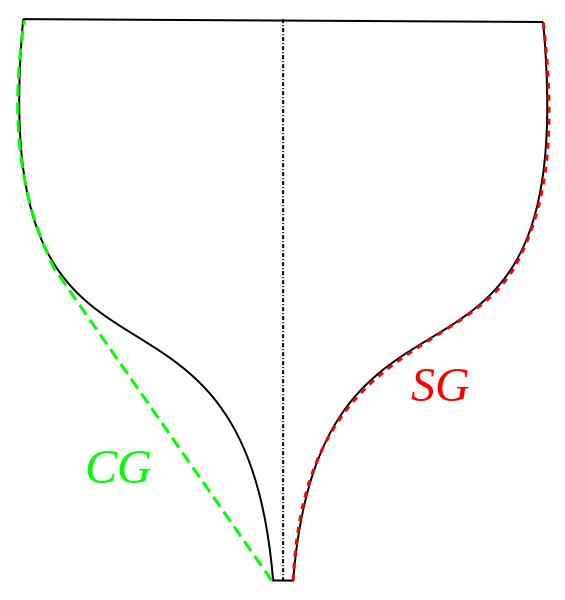
\includegraphics[width=5cm, height=5cm]{img/catena}
				\caption{Differenza tra catena CG (chain girth) e contorno SG (skin girth), la linea orizzontale mostra la waterline}
				\label{fig:catena&contorno}
			\end{figure}
			
			La catena è una curva ideale che unisce la falchetta con il punto di massima immersione, mentre il contorno segue appunto il contorno della carena, le misure sono prese dal piano di galleggiamento. (verificare)
			Il bordo libero è invece l'altezza dell'opera morta.
			
			Successivamente affinamenti hanno portato alla formula definitiva ancora oggi in vigore (\ref{eq:int1933}).
			
				\begin{center}
					\begin{equation}
					R=\frac{L+\frac{1}{4}G+2D+\sqrt{SA}-F }{2,5}
					\label{eq:int1919}
					\end{equation}
				\end{center}
				
				\begin{center}
					\begin{equation}
					R=\frac{L+2D+\sqrt{SA}-F }{2,37}
					\label{eq:int1933}
					\end{equation}
				\end{center}
					
			\subsection{In America}
			
			\subsection{Lo IOR: una Regola Mondiale}
					
			\subsection{Conclusioni}
				Questo capitolo dimostra che l'evoluzione dello yacht non è dipesa solo e soltanto dalla ricerca della perfezione e della prestazione, ma in generale ha seguito quelli che erano i buchi disponibili nei regolamenti per permettere di fare la barca più veloce di un'altra, piuttosto che la barca perfetta. D'altro canto le numerose formule di stazza partorite dimostrano che non è facile trovare quali e in che misura i parametri di uno scafo influiscono sulle prestazioni: ogni condizione di vento e di mare avrà la sua forma preferita, sta al designer trovare la soluzione tecnologica che permetta al suo prodotto di destreggiarsi meglio nelle condizioni di mare ipotizzate lavorando all'interno di un particolare regolamento.
			
			